\subsubsection{Minuta de reunião (05-Novembro-2015)}

\begin{tabbing}
  Local \= xxx \kill
  Local \> : LEAD \\
  Data  \> : 05 de Novembro de 2015 \\
  Hora  \> : 13:00
\end{tabbing} 

%---------------------------------------------------------------------
\participantes{
  \gabriel,
  \julia,
  \estevão,
  \elael,
  \renan,
  \ramon.

}

\textbf{Aprovação da minuta}

\textbf{Update semanal do Projeto EMMA}
   									
						
\textbf{\gabriel.} 
	\begin{itemize}
			\item Agilizar a compra do sensor a Laser da empresa Faro.
			\item Trabalho em andamento do com Nuvem de Pontos e PCL.
			\end{itemize}
		
		\item \textbf{Novas tarefas:}
			\begin{itemize} 
				\item Entrar em contato com laboratório da UFRJ que está fazendo trabalho
				com solda.
			\end{itemize}

					
			
   \textbf{\estevão.} 
	\begin{itemize}
		\item \textbf{Tarefas concluídas:}
			\begin{itemize}    
			    \item Formalizou modificações do conceito de base para escotilha
			    inferior, previsto na última reunião.
				
			\end{itemize}
		
		\item \textbf{Novas tarefas:}
			\begin{itemize} 
			    \item Agilizar a compra de Motoman, entrar em contato e verificar
			    se configuração que queremos é possível.
			    \item Formalizar conceito no Journal do EMMA.
			\end{itemize}
	\end{itemize}

	
	  \textbf{\elael.} 
	\begin{itemize}
		\item \textbf{Tarefas concluídas:}
			\begin{itemize}    
				\item Relatório técnico do teste do sensor da Faro.
				\item Entrar em contato com laboratório da UFRJ que está fazendo trabalho
				com esmerilhamento.
			\end{itemize}
		
		\item \textbf{Novas tarefas:}
			\begin{itemize} 
			    \item Formalizar descobertas do teste de sensores no Journal do EMMA.
			\end{itemize}
	\end{itemize}			
			
  \textbf{\renan.} 
	\begin{itemize}
		\item \textbf{Tarefas concluídas:}
			\begin{itemize}    
				\item Trabalhando no modelo de pá gerada através da nuvem de pontos do
				sensor a laser da empresa Faro.
			\end{itemize}
		
		\item \textbf{Novas tarefas:}
			\begin{itemize} 
			    \item Formalizar descobertas do teste de sensores no Journal do EMMA.
			\end{itemize}
	\end{itemize}	
			
   \textbf{\julia.} 
	\begin{itemize}
		\item \textbf{Tarefas concluídas:}
			\begin{itemize}    
				\item Análise de Tarefas da Calibração.
				\item Estudo de processos que podem ser aplicados na construção do software,
				possíveis problemas e possibilidades de arquitetura de informação.
			\end{itemize}
		
		\item \textbf{Novas tarefas:}
			\begin{itemize} 
			    \item Possibilidades para análise de tarefas de outras atividades
			    (hardcoating e planejamento de trajetória).
			\end{itemize}
	\end{itemize}		



\textbf{Agenda para a próxima reunião:}
  \begin{itemize}
    \item Resultado de pesquisas individuais.
    \item Novas tarefas \& recomendações.
  \end{itemize}


\vspace{5mm}%
\parbox[t]{70mm}{ 
  Aprovado por: \\[5mm]
  \centering
  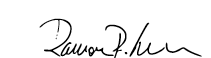
\includegraphics[width=65mm]{figs/logo/assinatura-ramon.png} \\[-4mm]
  \rule[2mm]{70mm}{0.1mm} \\
  \ramon \\[1mm]
  Coordenador do Projeto \\
}

%---------------------------------------------------------------------
\fim